\documentclass{article}
\usepackage{graphicx} % Required for inserting images
\usepackage{tikz}
\usetikzlibrary {arrows.meta} 
\usepackage{tikz-3dplot}
\usepackage{tikz}
\usepackage[a4paper,top=1.5cm,left=2.5cm,right=2.5cm,bottom=2cm]{geometry}
\usepackage{amsmath}

\title{tickz_sandbox}
\author{lucasguedes778 }
\date{October 2023}

\begin{document}
% \section{Introduction}

% \begin{tikzpicture}

% % Poligono grande da esquerda
% \draw (3.64, 6.73) -- (7.34,5.97) -- (5.616,1.91) -- (2.51,1.91) -- (0.729,4.73) -- (3.64, 6.73);

% % Poligono grande da direita
% \draw (4.401, 5.08) -- (8.586, 7.7) -- (13.58, 2.28) -- (8.1, 1.29) -- (4.401, 3.2) -- (4.401, 5.08);

% % Poligono preenchido com amarelo

% \fill[yellow] (5.185, 5.55) -- (5.91, 4.81) -- (5.67, 3.06) -- (4.4, 3.60) -- (4.4, 5.08) -- (5.185, 5.58);

% % Poligono que faz interseccao entre os dois maiores
% \draw (4.698, 6.03) -- (5.91, 4.81) -- (5.67, 3.06) -- (2.268, 4.55) -- (4.698, 6.03);

% % Seta para cima - Vara
% \draw[->] (14.121, 0.067) -- (14.121, 7.37); 

% \draw (14.121, 6.22) -- (6.230, 6.22);
% \draw (14.121, 5.57) -- (5.198, 5.57);
% \draw (14.121, 4.95) -- (5.198, 4.95);

% % Setas espalhadas ao longo da figura
% \draw[->] (7.155, 3.06) -- (4.995, 4.06);
% \draw[->] (10.638, 7.43) -- (9.42, 6.94);
% \draw[->] (3.942, 1.4) -- (3.726, 4.52);
% \draw[->] (1.62, 0.8) -- (1.458, 4.55);
% \draw[->] (1.215, 6.56) -- (2.187, 6.05);
% \draw[->] (8.91, 1.199) -- (8.694, 2.1);

% \node[text width=4cm] at (3.9,0.78) {$\{x | Cx \leq d\}$};
% \node[text width=4cm] at (6,1.373) {$Co\{x \in X | Cx \leq d\}$};
% \node[text width=4cm] at (11,1.211) {$\{x | Ax \leq b\}$};
% \node[text width=4cm] at (9.5,2.611) {$\{Co\{x \in X | Cx \leq d\}$};
% \node[text width=4cm] at (9.5,3) {$\{x|Ax \leq b\}\cap$};

% \node[text width=4cm] at (15,5.196) {$v(P)$};
% \node[text width=4cm] at (15,5.8) {$v(PR)$};
% \node[text width=4cm] at (15,6.4) {$v(PL)$};


% \node[text width=4cm] at (12,7.83) {\textbf{RELAX}};
% \node[text width=4cm] at (2.5,7) {\textbf{KEEP}};

% \node[text width=4cm] at (4.05,4.55) {x};
% \node[text width=4cm] at (7.7,3) {x};
% \node[text width=4cm] at (6.9,5) {x};
% \node[text width=4cm] at (6,5.2) {x};
% \node[text width=4cm] at (6.5,6.2) {x};
% \node[text width=4cm] at (11,4.5) {x};
% \node[text width=4cm] at (14,3) {x};


% \node[text width=4cm] at (16.5,7) {$f$};

% \end{tikzpicture}


\tdplotsetmaincoords{45}{45}


\begin{tikzpicture}[tdplot_main_coords,thick, scale=0.9]

\draw (0,0,0) -- (0,9,0) -- (15, 9, 0) -- (15, 0, 0) --  (0,0,0);

% Poligono grande da esquerda
\draw (3.64, 6.73, 0) -- (7.34,5.97, 0) -- (5.616,1.91, 0) -- (2.51,1.91, 0) -- (0.729,4.73, 0) -- (3.64, 6.73, 0);

% Poligono grande da direita
\draw (4.401, 5.08, 0) -- (8.586, 7.7, 0) -- (13.58, 2.28, 0) -- (8.1, 1.29, 0) -- (4.401, 3.2, 0) -- (4.401, 5.08, 0);

% Poligono preenchido com amarelo

\fill[yellow] (5.185, 5.55, 0) -- (5.91, 4.81, 0) -- (5.67, 3.06, 0) -- (4.4, 3.60, 0) -- (4.4, 5.08, 0) -- (5.185, 5.58, 0);

% Poligono que faz interseccao entre os dois maiores
\draw (4.698, 6.03, 0) -- (5.91, 4.81, 0) -- (5.67, 3.06, 0) -- (2.268, 4.55, 0) -- (4.698, 6.03, 0);

% Seta para cima - Vara
% \draw[->] (14.121, 0.067, 0) -- (14.121, 7.37, 0); 

% \draw (14.121, 6.22, 0) -- (6.230, 6.22, 0);
% \draw (14.121, 5.57, 0) -- (5.198, 5.57, 0);
% \draw (14.121, 4.95, 0) -- (5.198, 4.95, 0);

% Setas espalhadas ao longo da figura
\draw[->] (7.155, 3.06, 0) -- (4.995, 4.06, 0);
\draw[->] (10.638, 7.43, 0) -- (9.42, 6.94, 0);
\draw[->] (3.942, 1.4, 0) -- (3.726, 4.52, 0);
\draw[->] (1.62, 0.8, 0) -- (1.458, 4.55, 0);
\draw[->] (1.215, 6.56, 0) -- (2.187, 6.05, 0);
\draw[->] (8.91, 1.199, 0) -- (8.694, 2.1, 0);

\node[text width=4cm] at (3.9,0.78, 0) {$\{x | Cx \leq d\}$};
\node[text width=4cm] at (6,1.373, 0) {$Co\{x \in X | Cx \leq d\}$};
\node[text width=4cm] at (11,1.211, 0) {$\{x | Ax \leq b\}$};
\node[text width=4cm] at (9.5,2.611, 0) {$\{Co\{x \in X | Cx \leq d\}$};
\node[text width=4cm] at (9.5,3, 0) {$\{x|Ax \leq b\}\cap$};

\node[text width=4cm] at (15,5.196, 0) {$v(P)$};
\node[text width=4cm] at (15,5.8, 0) {$v(PR)$};
\node[text width=4cm] at (15,6.4, 0) {$v(PL)$};


\node[text width=4cm] at (12,7.83, 0) {\textbf{RELAX}};
\node[text width=4cm] at (2.5,7, 0) {\textbf{KEEP}};

\node[text width=4cm] at (4.05,4.55, 0) {x};
\node[text width=4cm] at (7.7,3, 0) {x};
\node[text width=4cm] at (6.9,5, 0) {x};
\node[text width=4cm] at (6,5.2, 0) {x};
\node[text width=4cm] at (6.5,6.2, 0) {x};
\node[text width=4cm] at (11,4.5, 0) {x};
\node[text width=4cm] at (14,3, 0) {x};


% \node[text width=4cm] at (16.5,7, 0) {$f$};

% Setas que saem do plano
\draw[ultra thick,-{Circle[]}] (6.291, 6.21, 0) -- (6.291, 6.21, 4); 

\draw[ultra thick,-{Circle[]}] (5.150, 5.6, 0) -- (5.150, 5.6, 5.5); 

\draw[ultra thick,-{Circle[]}] (5.18, 4.95, 0) -- (5.18, 4.95, 7); 

% Plano superior
\draw[fill=blue, draw=blue, fill opacity=0.5] (2, 7, 2) -- (12, 7, 2) -- (12, 4, 9.5) -- (2, 4, 9.5) -- (2, 7, 2);

\end{tikzpicture}

\newpage

\section{Replicar exemplo 1-tree TSP Wolsey (Cap 10) (matrizes e figuras da solução)}

\[(c_e) = 
\begin{bmatrix}
- & 30 & 26 & 50 & 40\\
- & - & 24 & 40 & 50 \\
- & - & - & 24 & 26 \\
- & - & - & - & 30 \\
- & - & - & - & - 
\end{bmatrix}
\]


\[(\overline{c}_e) = 
\begin{bmatrix}
- & 30 & 41 & 50 & 40\\
- & - & 39 & 40 & 50 \\
- & - & - & 39 & 26 \\
- & - & - & - & 30 \\
- & - & - & - & - 
\end{bmatrix}
\]


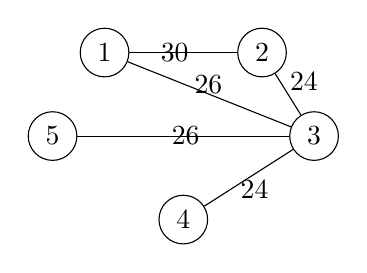
\begin{tikzpicture}[node distance={15mm}, main/.style = {draw, circle}] 
\node[main] (5) {$5$}; 
\node[main] (1) [above right of=5, xshift=-4mm] {$1$};
\node[main] (2) [right of=1, xshift=5mm] {$2$}; 
\node[main] (3) [below right of=2, xshift=-4mm] {$3$};
\node[main] (4) [below left of=3, xshift=-6mm] {$4$};

\draw (5) -- (3) node [midway, below, right, pos=0.4] {26};
\draw (3) -- (4) node [midway, below, right, pos=0.7] {24};
\draw (1) -- (3) node [midway, above, right, pos=0.35] {26};
\draw (1) -- (2) node [midway, above, right, pos=0.2] {30};
\draw (2) -- (3) node [midway, above, right, pos=0.2] {24};

\end{tikzpicture} 

\section{Duas subfiguras com exemplos de cortes em um grafo (em uma delas, S deve 
estar separado, à esquerda de S', e na outra, os nós de S e S' devem estar misturados}


\begin{center}
    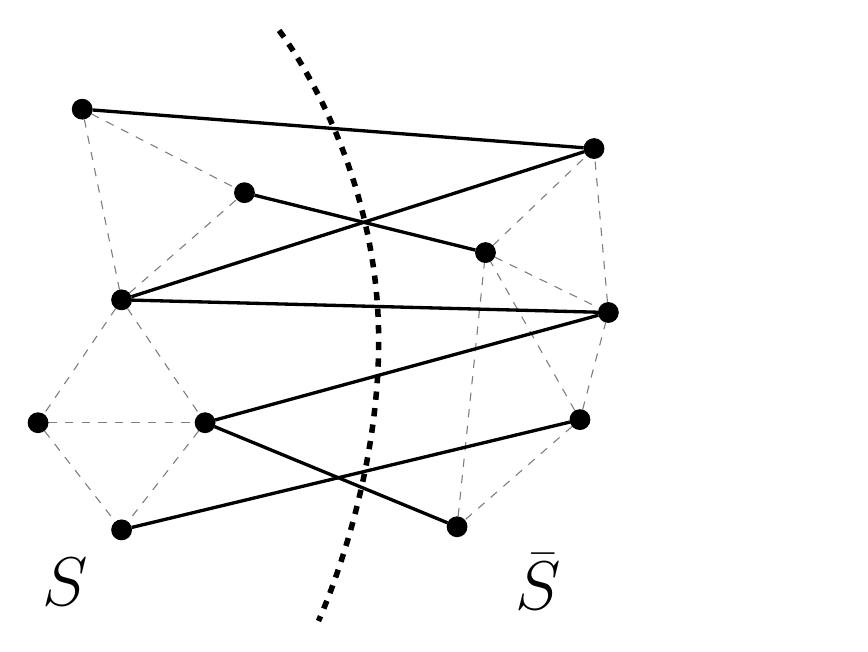
\begin{tikzpicture}[node distance={15mm}, main/.style = {draw, circle, fill=black, inner sep = 0, minimum size = 0.25cm}] 
    
% \draw[fill=black!20, fill opacity=0.5, draw=black!70, dashed] (0.7,-2.5) ellipse (2cm and 3.5cm);
% \draw[fill=black!20, fill opacity=0.5, draw=black!70, dashed] (5.4,-2.5) ellipse (2cm and 3.7cm);


\node[main] (1) {};
\node[main] (2) [right of=1, xshift=50mm, yshift=-5mm]{};
\node[main] (3) [below right of=1, xshift=10mm]{};
\node[main] (4) [below right of=3, xshift=20mm, yshift=3mm]{};
\node[main] (5) [below right of=4, xshift=5mm, yshift=3mm]{};
\node[main] (7) [below left of=3, xshift=-5mm, yshift=-3mm]{};
\node[main] (8) [below left of=7, yshift=-5mm]{};
\node[main] (9) [below right of=8, yshift=-3mm]{};
\node[main] (10) [above right of=9, yshift=3mm]{};
\node[main] (11) [below left of=5, yshift=-3mm, xshift=7mm]{};
\node[main] (12) [below left of=11, yshift=-3mm, xshift=-5mm]{};


\draw[very thick] (1) -- (2) node [midway, below, right, pos=0.4] {};
\draw[very thick] (3) -- (4) node [midway, below, right, pos=0.4] {};
\draw[very thick] (7) -- (2) node [midway, below, right, pos=0.4] {};
\draw[very thick] (7) -- (5) node [midway, below, right, pos=0.4] {};
\draw[very thick] (10) -- (5) node [midway, below, right, pos=0.4] {};
\draw[very thick] (10) -- (12) node [midway, below, right, pos=0.4] {};
\draw[very thick] (9) -- (11) node [midway, below, right, pos=0.4] {};

\draw[dashed, opacity = 0.5] (1) -- (3) node [midway, below, right, pos=0.4] {};
\draw[dashed, opacity = 0.5] (1) -- (7) node [midway, below, right, pos=0.4] {};
\draw[dashed, opacity = 0.5] (7) -- (3) node [midway, below, right, pos=0.4] {};
\draw[dashed, opacity = 0.5] (7) -- (8) node [midway, below, right, pos=0.4] {};
\draw[dashed, opacity = 0.5] (7) -- (10) node [midway, below, right, pos=0.4] {};
\draw[dashed, opacity = 0.5] (10) -- (9) node [midway, below, right, pos=0.4] {};
\draw[dashed, opacity = 0.5] (8) -- (9) node [midway, below, right, pos=0.4] {};
\draw[dashed, opacity = 0.5] (11) -- (12) node [midway, below, right, pos=0.4] {};
\draw[dashed, opacity = 0.5] (11) -- (4) node [midway, below, right, pos=0.4] {};
\draw[dashed, opacity = 0.5] (12) -- (4) node [midway, below, right, pos=0.4] {};
\draw[dashed, opacity = 0.5] (4) -- (5) node [midway, below, right, pos=0.4] {};
\draw[dashed, opacity = 0.5] (11) -- (5) node [midway, below, right, pos=0.4] {};
\draw[dashed, opacity = 0.5] (5) -- (2) node [midway, below, right, pos=0.4] {};
\draw[dashed, opacity = 0.5] (4) -- (2) node [midway, below, right, pos=0.4] {};
\draw[dashed, opacity = 0.5] (8) -- (10) node [midway, below, right, pos=0.4] {};

% \draw[dashed, color=red] (0.7,-2.5) ellipse (2cm and 3.5cm);
% \draw[dashed, color=blue] (5.2,-2.5) ellipse (2cm and 3.7cm);

 \node[text width=4cm, color=black] at (1.5,-6) {\Huge $S$};
\node[text width=4cm, color=black] at (7.5,-6) {\Huge $\bar{S}$};

\draw[dashed, line width = 2pt] plot[smooth, tension=1] coordinates { (2.5, 1) (3.75, -2.5) (3, -6.5) };


\end{tikzpicture} 
\end{center}

\end{document}
